Currently, ATLAS deploys 20 instances of the PanDA Broker on 4 Titan's DTNs, 5
instances per DTN. Each broker submits and manages the execution of 15 to 300
ATLAS jobs, one job for each worker node, and a theoretical maximum concurrent
use of 96,000 cores. Since November 2015, PanDA Brokers have operated only in
backfill mode, without a defined time allocation, and running at the lowest
priority on Titan.

We evaluate the efficiency, scalability and reliability of the deployment of PanDA WMS on Titan by characterizing the behavior of both PanDA Broker and AthenaMP.
% two dimensions: (i) backfill utilization by the PanDA Brokers; and (ii) the
% amount of runtime spent performing detector simulations.
We based our characterizations on measuring the number of cores utilized by
ATLAS on Titan, the overall backfill availability, the number of detector
simulations performed on all the resources available to ATLAS and on Titan, and
the failure rate of these simulations. We also consider the the time taken to
setup AthenaMP and to simulate events in the ATLAS detector with it. All the
measurements were performed between January 2016 and February 2017, hereafter
called `experiment time window'.

\mtnote{TODO: expand the previous paragraph to include dimensions of AthenaMP characterization.}

% -----------------------------------------------------------------------------
\subsection{Characterizing the PanDA Broker on Titan}
\label{ssec:panda_titan}

Figure~\ref{fig:backfill-utilization} (gray bars) shows the number of
core-hours used by ATLAS during the experiment time window. ATLAS consumed a
total of 73.8M core-hours, for an average of $\approx$7M core-hours a month,
with a minimum of 3.3M core-hours in April 2016 and a maximum 14.8M core-hours
in February 2017.

\begin{figure}[htp]
    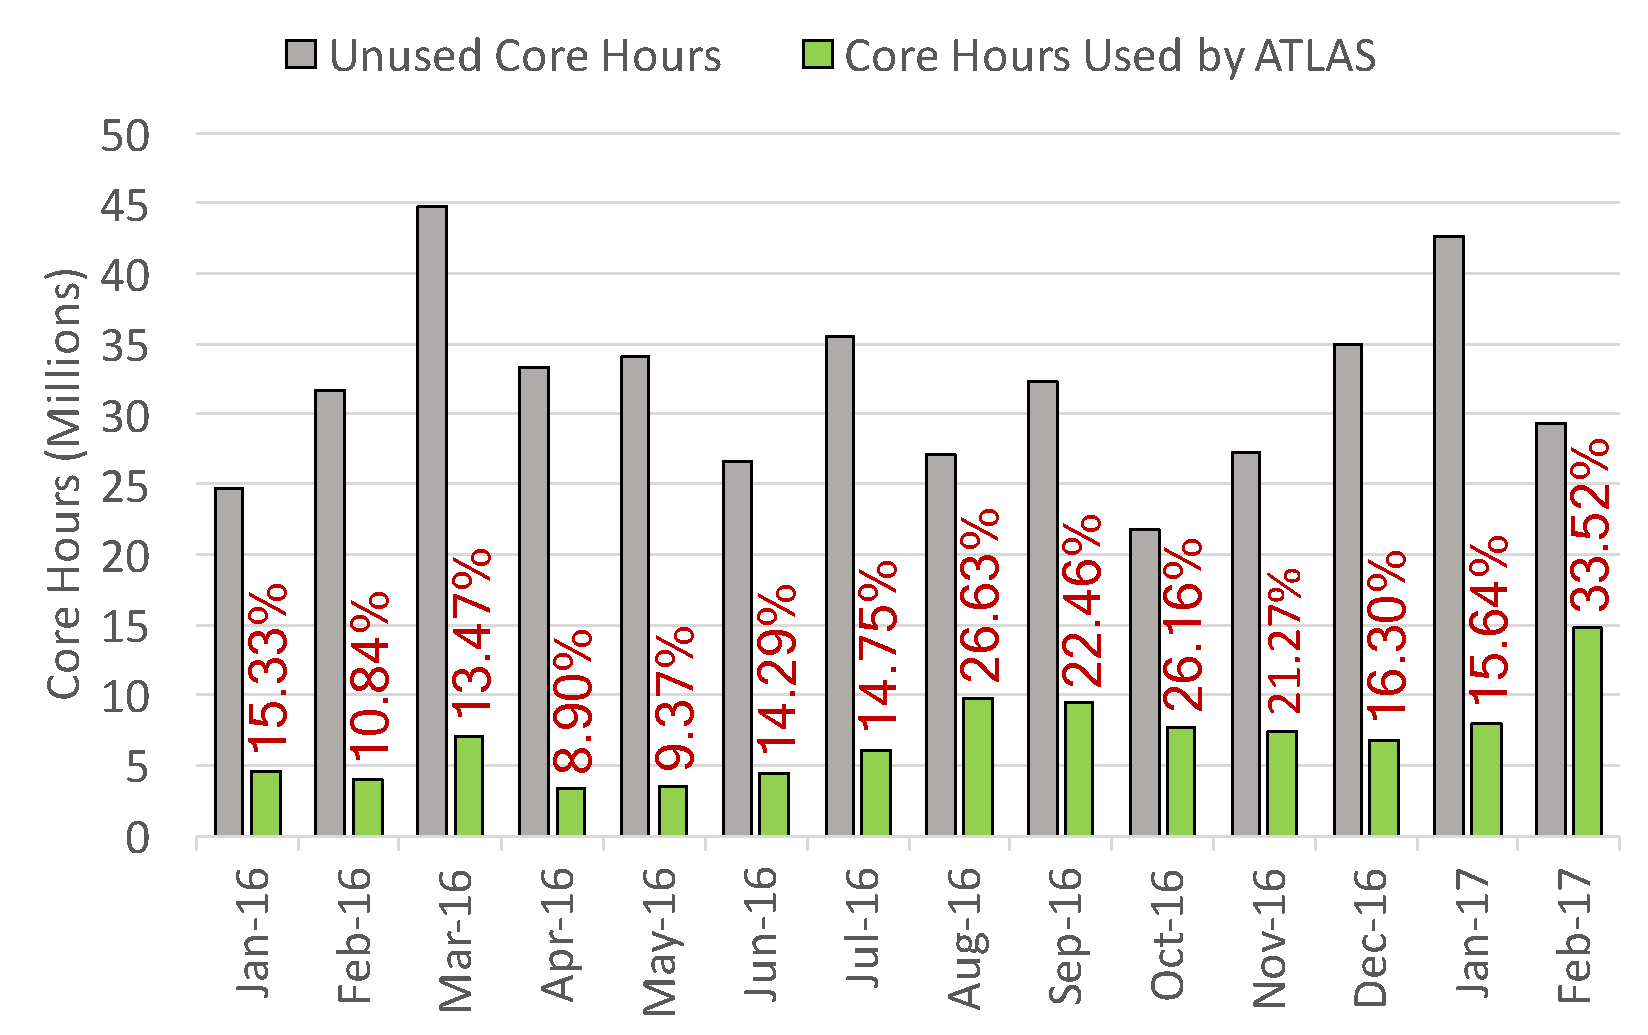
\includegraphics[clip,width=\columnwidth]{figures/backfill_consumption.pdf}
    \caption{Gray bars: Number of unused cores of Titan's backfill availability;
    blue bars: Number of cores of Titan's backfill availability used by ATLAS
    via PanDA Brokers; red labels: Efficiency of PanDA Brokers defined as
    percentage of Titan's backfill availability used by ATLAS.}
\label{fig:backfill-utilization}
\end{figure}

Figure~\ref{fig:backfill-utilization} (green bars) shows backfill utilization
during the experiment time window.  Efficiency
(Figure~\ref{fig:backfill-utilization}, red labels) is defined as the fraction
of Titan core-hours utilized by the PanDA Brokers (for ATLAS jobs) to the total
of Titan’s backfill availability. The brokers reached 18\% average efficiency,
with a minimum 8.9\% efficiency on April 2016 and a maximum 33.5\% efficiency on
February 2017. The total backfill available was 38.1M Titan core-hours in April
2016, and 33.1M Titan core-hours in February 2017. This shows that the measured
difference in efficiency did not depend on a comparable difference in total
backfill availability.

\mtnote{Elaborate further and put it at the end, after giving several of the
measurements we would need. ``Currently, this measure of efficiency is being
refined on the base of the actual minimum amount of walltime that PanDA Broker
can request when submitting job requests. This is not a fixed value as it
depends on variable initialization and configuration overheads, simulation time,
and number of nodes obtained. Part of the undergoing effort is to enable the
measurements of  the distribution of these parameters to derive an optimization
function.''}

\jhanote{I would plot the efficiency on the Y2 axis for both
[diagrams].}\mtnote{Done but then the first diagram ended up plotting a subset
of the data of the second diagram. I used only the second diagram.} \jhanote{I
would suggest similar style of X-axis as previous figure. Difficult to parse
which is April if we are going to call out a specific month. Also consistency in
style is generally good to keep cognitive burden low.}\mtnote{Done.}

% Figure~\ref{fig:hpc-workload-utilization} shows that d

During the experiment time window, about 2.25M detector simulation jobs were
completed on Titan, for a total of 225M events processed. This is equivalent to
0.9\% of all the 250M detector simulations performed by ATLAS in the same period
of time, and 3.5\% of the 6.6B events processed by those jobs. Comparatively,
Titan contributed 3.9\% of the total of around 200K cores available to ATLAS on
Grid, Cloud, and HPC infrastructures together. These figures confirms the
relevance of supercomputers' resource contribution to the LHC Run 2, especially
when accounting for the amount of unused backfill availability and the
improvement of PanDA efficiency across the experiment time window.

% \begin{figure}[htp]
%     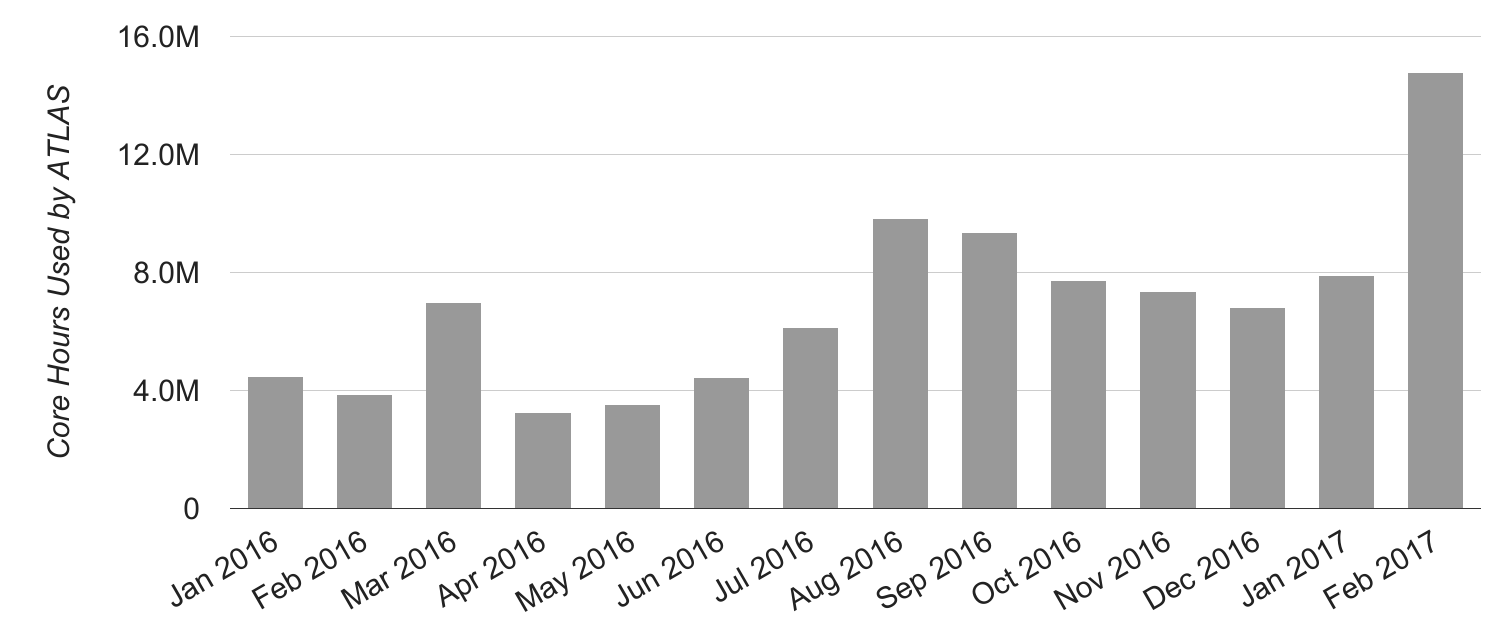
\includegraphics[clip,width=\columnwidth]{figures/cpu_hours.png}
% \caption{\mtnote{Placeholder for the diagram/data I asked to Danila and
% Sergey. Consider a table instead of a figure.}}
% \label{fig:hpc-workload-utilization}
% \end{figure}

On February 2017, PanDA Brokers used almost twice as much backfill availability
than in any other month. No relevant code update was made during that period and
logs indicated that the brokers were able to respond more promptly to backfill
availability. This is likely due to hardware upgrades on the DTNs. The absence
of continuous monitoring of those nodes does not allow to quantify bottlenecks
but spot measurements of their load indicate that a faster CPU and better
networking were likely responsible for the improved performance.

Investigations showed an average CPU load of 3.6\% on the upgraded DTNs. As
such, further hardware upgrades seem unlikely to improve significantly the
performance of PanDA Brokers. Nonetheless, the current load suggests that the
number of brokers per DTN could be increased. This would enable the submission
of a larger number of concurrent jobs to Titan's PBS queue, allowing for PanDA
to consume a higher percentage of backfill availability.

Every detector simulation executed on Titan process 100 events. This number of
events is consistent with the physics of the use case and with the average
duration of backfill availability. The duration of a detector simulation is a
function of the number of events: the more events, the longer the simulation.
Not all events take the same time to be simulated:
% Figure~\ref{fig:100event-distrib} shows a distribution of the simulation time
% of
1 event takes from $\approx$2 to $\approx$40 minutes to be simulated, with a
mean of $\approx$14 minutes. Considering that each worker node process up to 16
events concurrently, 100 events takes around 2 hours to process.

% \begin{figure}[htp]
%     \includegraphics[clip,width=\columnwidth]{figures/tx_simulation_distribution.pdf}
%     \caption{Distribution of the time taken by a Geant4 detector simulation to
%     simulate one event. 3000 Events; 30 Titan worker nodes; 16 simulations per
%     node; 100 events per node. Average time per event $\approx$14 min. Broad
%     distribution from $\approx$2 to $\approx$40 minutes.}
% \label{fig:100event-distrib}
% \end{figure}

Figure~\ref{fig:backfill-distrib} shows the distribution of backfill
availability on Titan as a function of number of nodes and the time of their
availability (i.e., walltime). We recorded these data by polling Titan's Moab
scheduler at regular intervals during the experiment window time, while
developing and deploying PanDA Brokers. The mean number of nodes was 691, and
their mean walltime was 126 minutes. Detector simulations of 100 events, enable
to use down to 1 node for 1/2 of the mean walltime of backfill availability. As
such, it offers a good compromise for PanDA Broker efficiency.

\begin{figure*}%[htp]
    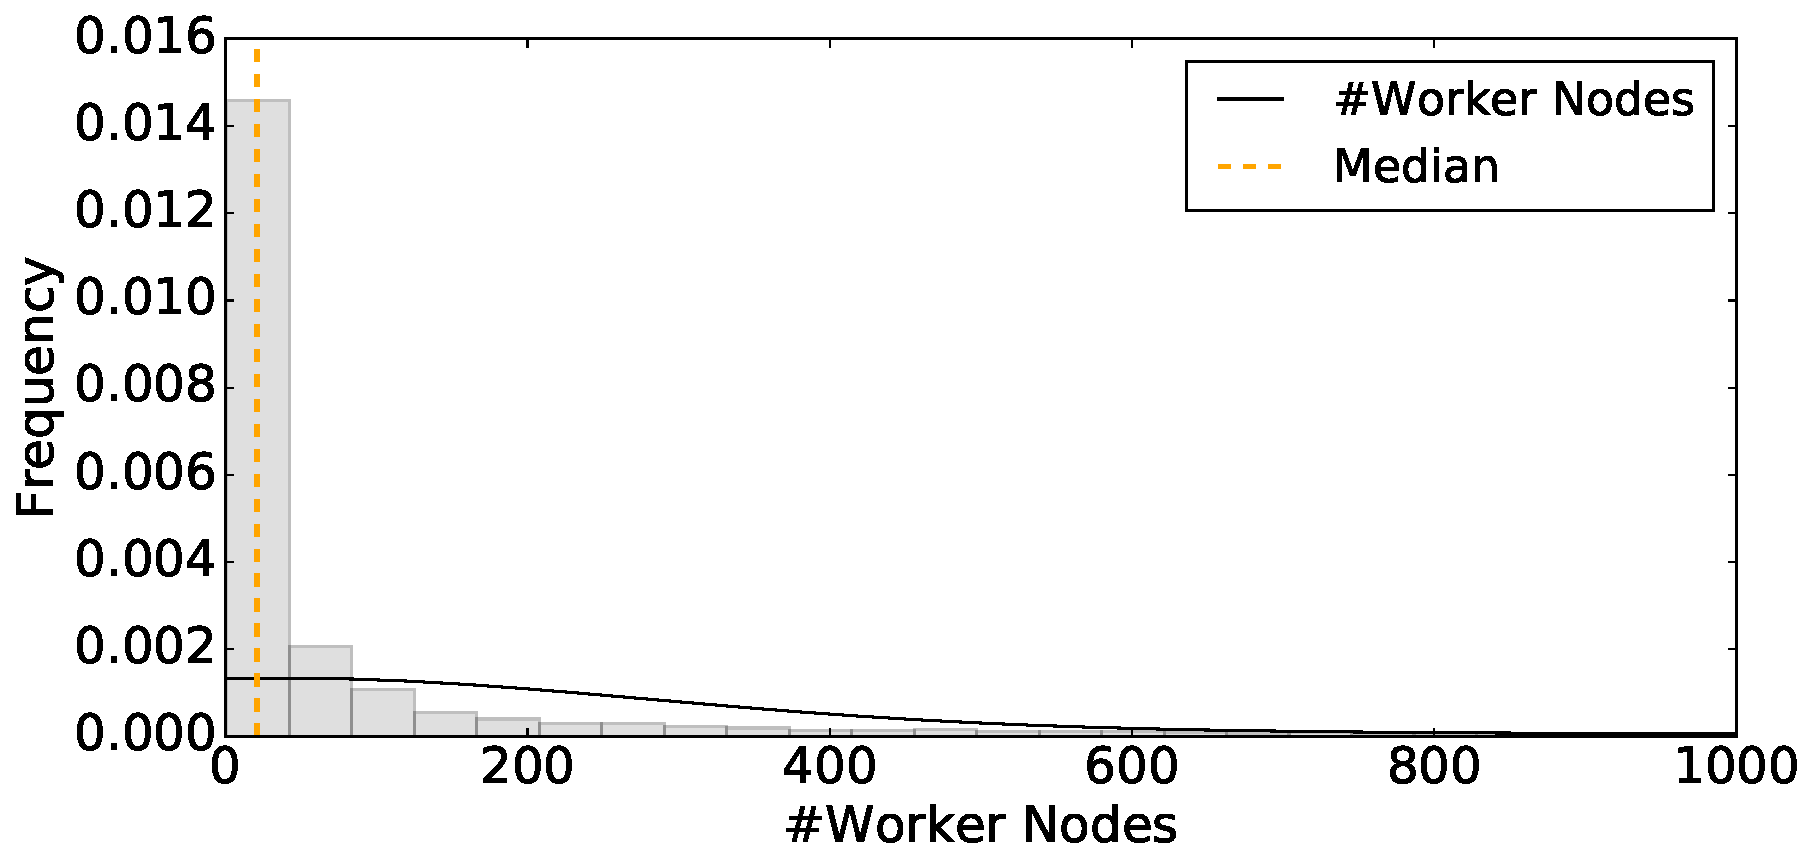
\includegraphics[clip,width=0.32\textwidth]{figures/titan_backfill_wnodes_distribution.pdf}
    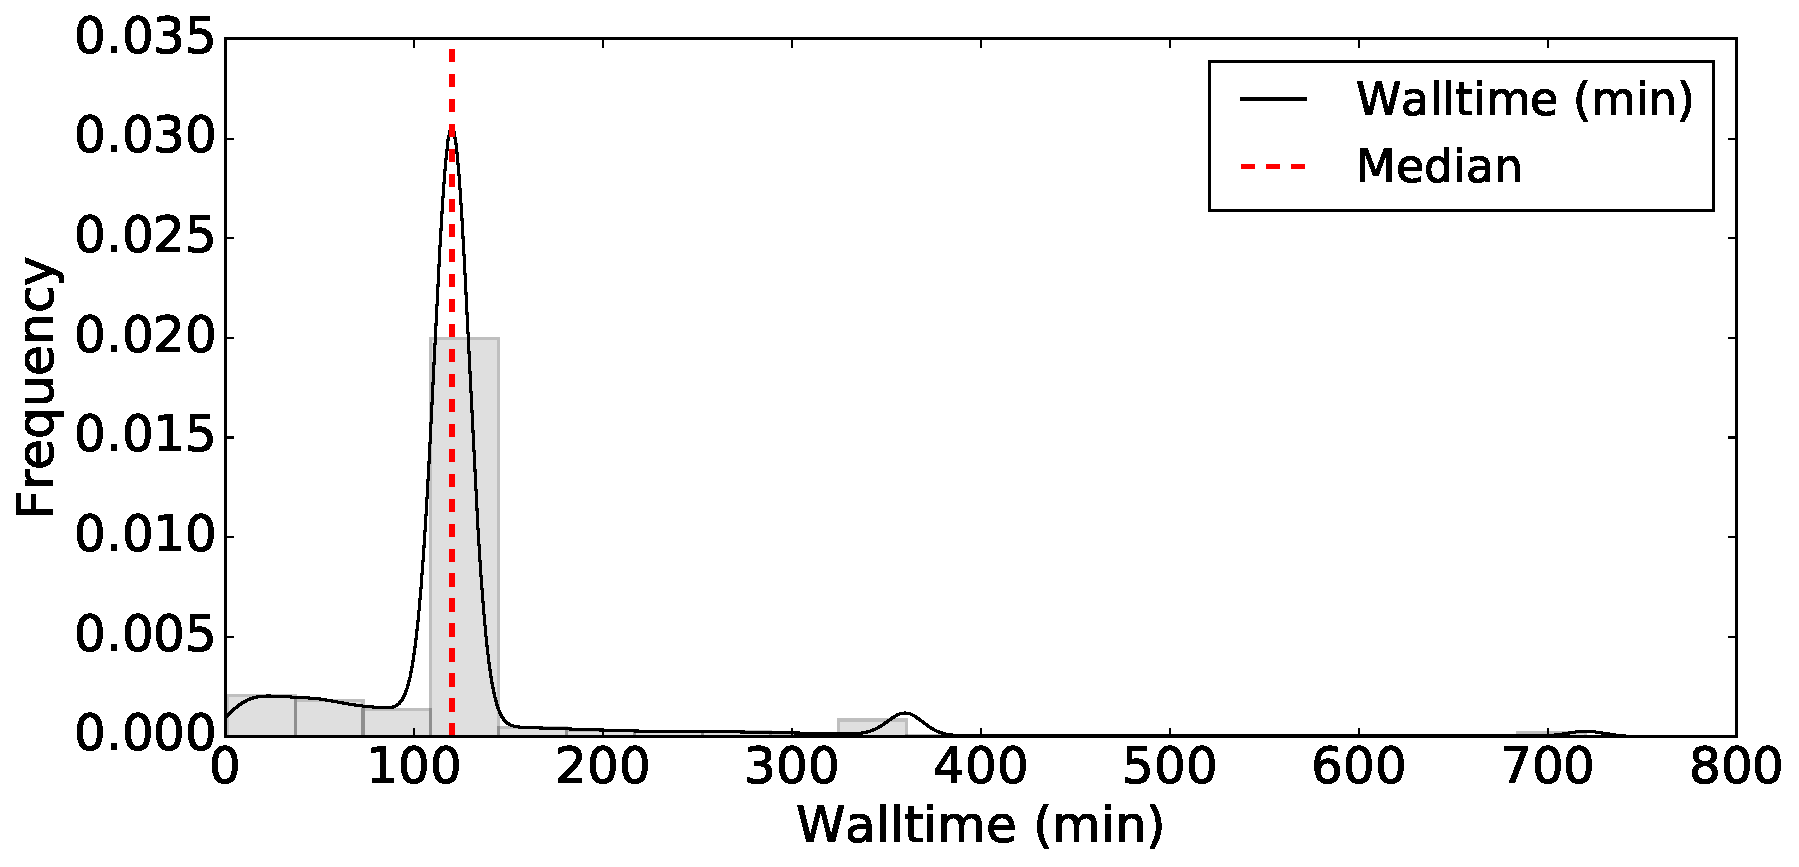
\includegraphics[clip,width=0.32\textwidth]{figures/titan_backfill_walltime_distribution.pdf}
    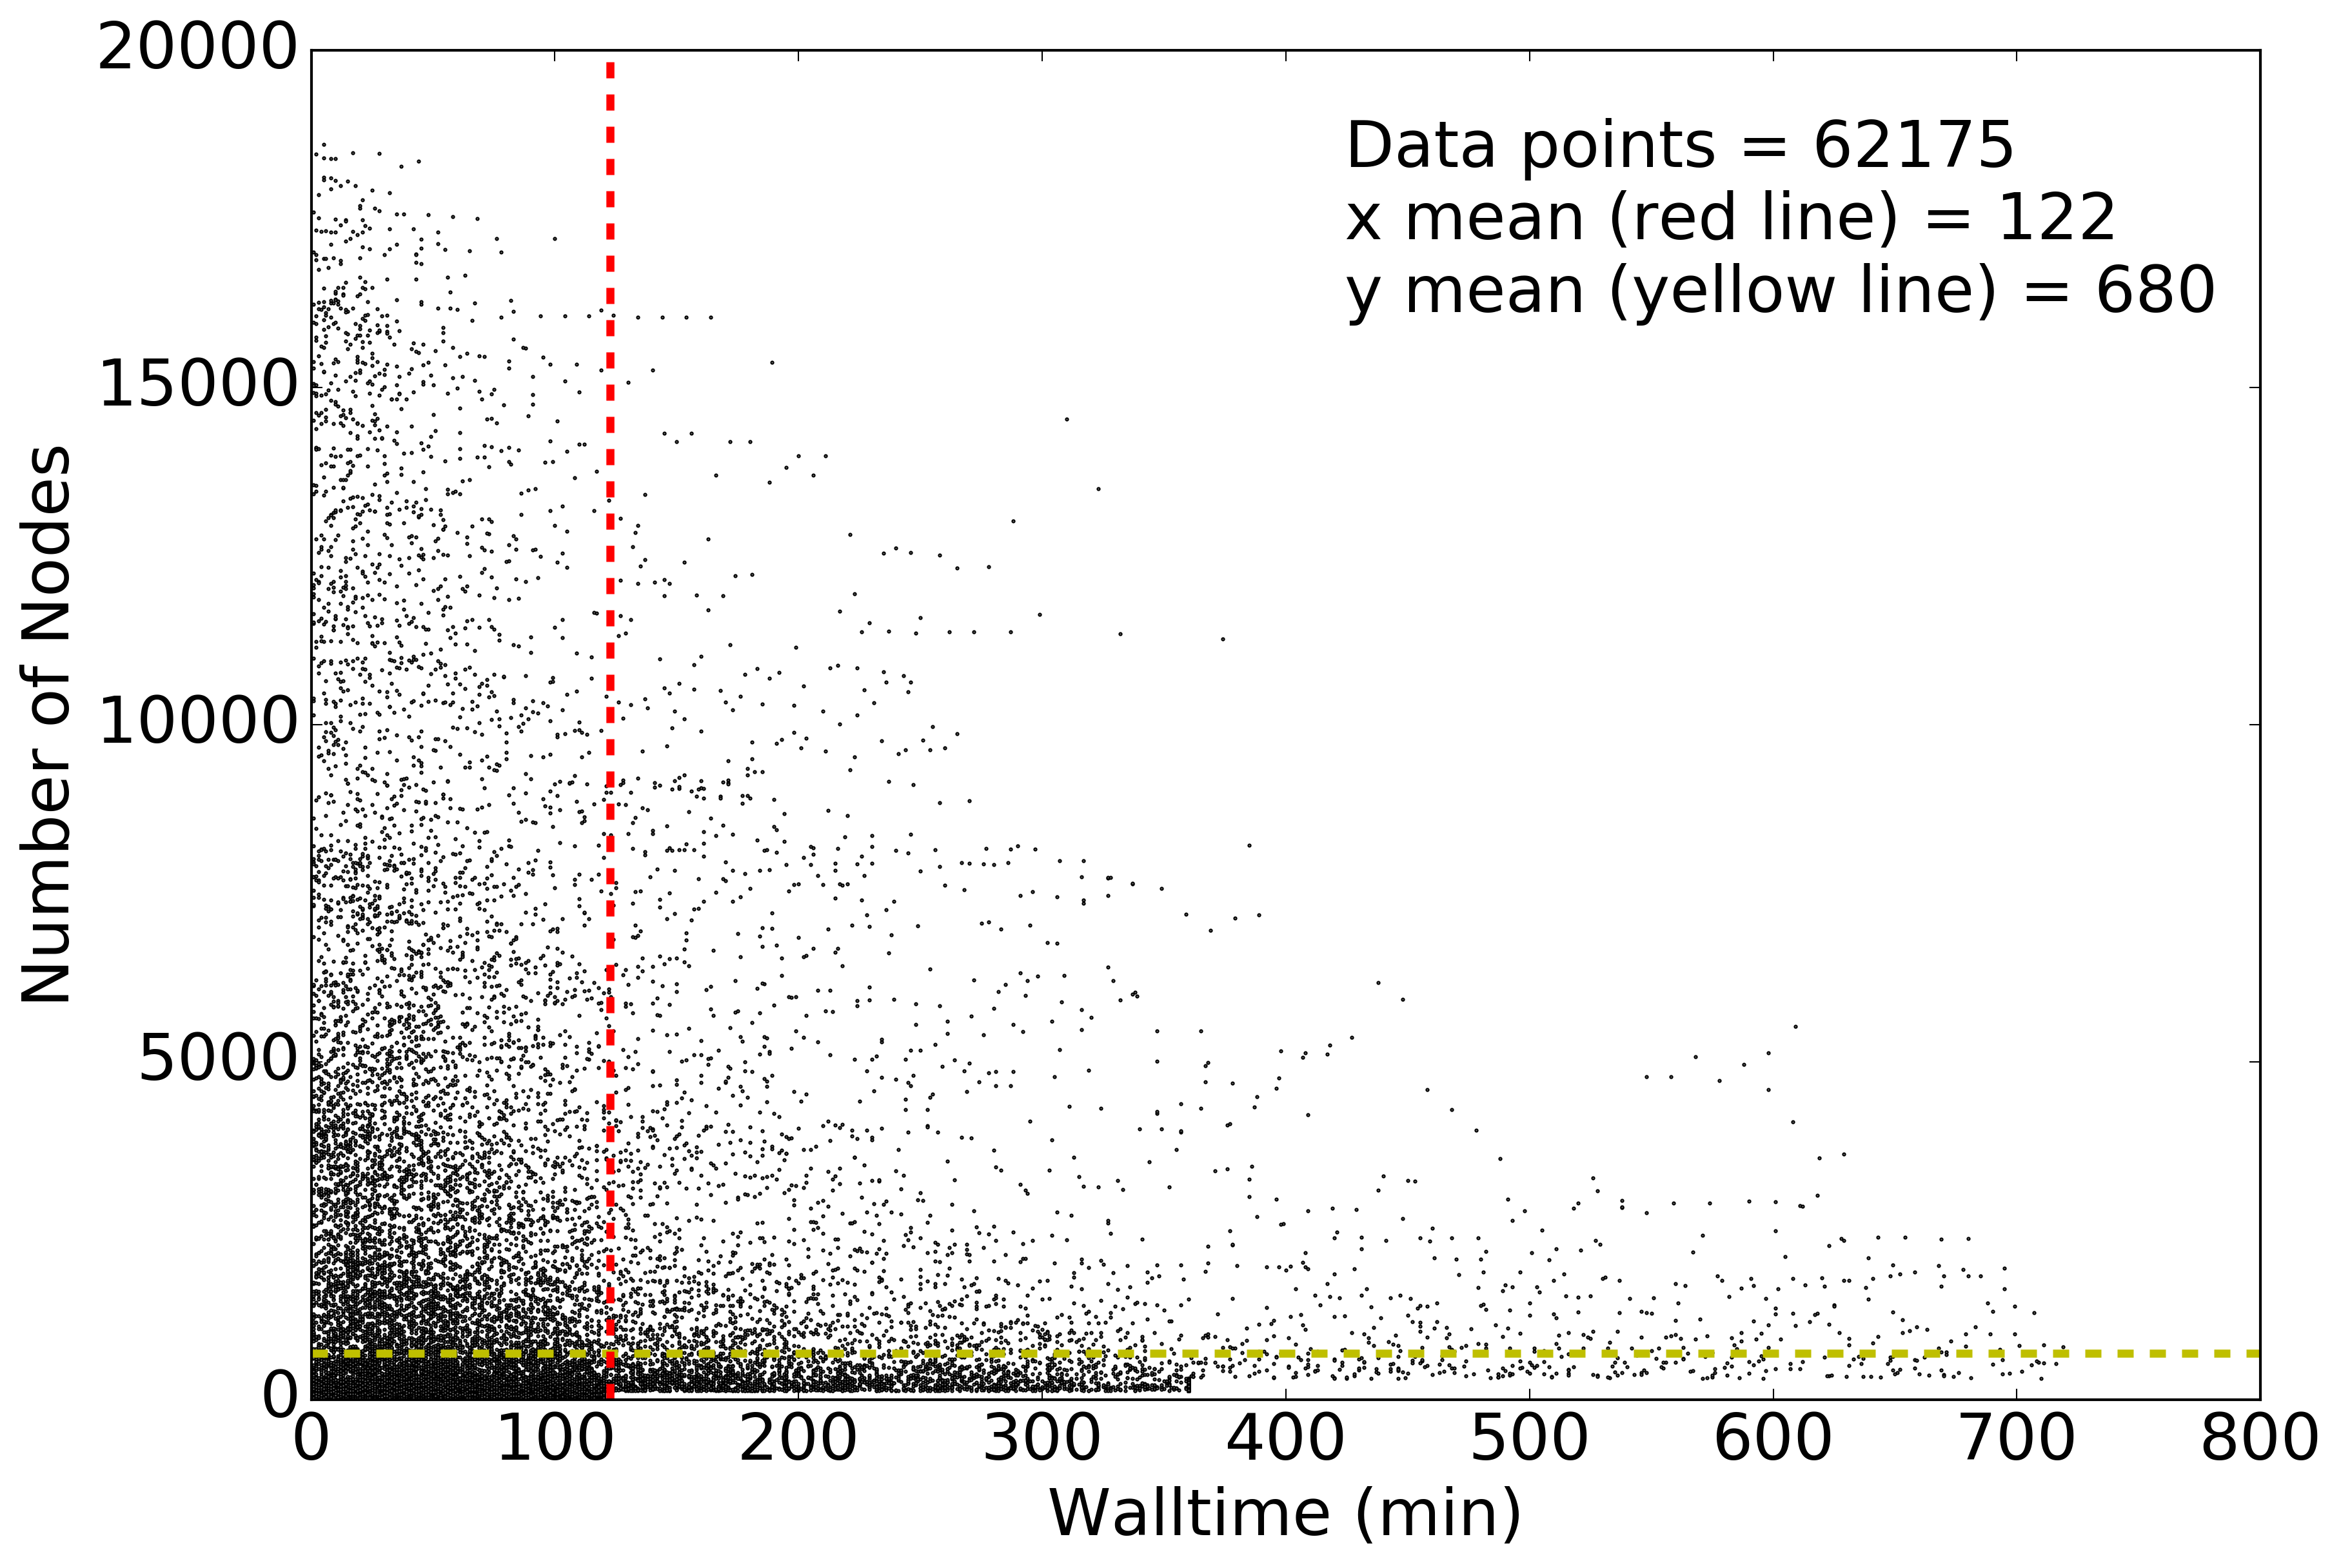
\includegraphics[clip,width=0.32\textwidth]{figures/titan_backfill_avail.png}
    %figures/avail_time_vs_nodes_Oct_28_Nov_3_2015.pdf}
    \caption{Backfill availability: distribution of number of work nodes (left); distribution of walltime in minutes (center); and their correlation (right). 62175 measures: mean number of work nodes available 691; mean
    walltime available 126 minutes.}
\label{fig:backfill-distrib}
\end{figure*}

Usually, detector simulations performed on the Grid process 10 times the number
of events than those on Titan. This explains the difference between the
percentage of detector simulations (9\%) and of events computed by those
simulations (3.9\%) on Titan. PanDA Broker could fit the number of events to the
walltime of the backfill availability on the base of the distributions of
Fig.~\ref{fig:backfill-distrib}. That specific number of event could then be
pulled from the PanDA Event service~\cite{calafiura2015atlas} and given as input
to one or more simulations. Once packaged into the MPI script submitted to
titan's PBS batch system, these simulations would better fit backfill
availability, increasing the efficiency of PanDA Brokers.

The transition from a homogeneous to a heterogeneous number of events per
detector simulation has implications for the application layer. An even number
of events across simulations makes it easier to partition, track and package
events across simulations, especially when they are performed on both the Grid
and Titan. A homogeneous number of events also helps to keep the size and
duration of other stages of the MC workflow (\S\ref{ssec:panda-titan}) more
uniform. Further analysis is needed to evaluate the trade offs between increased
efficiency of resource utilization and the complexity that would be introduced
at the application layer.

Currently, each PanDA Broker creates, submits, and monitor a single MPI PBS
script at a time. This design is inherited from PanDA Pilot where a single
process is spawn at a time to execute the payload. As a consequence, the
utilization of a larger portion of Titan's backfill availability depends on the
the number of concurrent PanDA Brokers instantiated on the DTNs: When all the 20
PanDA Brokers have submitted a MPI PBS Job, further backfill availability cannot
be used.

Based on the current data, increasing PanDA Brokers efficiency on Titan would
require around 60 concurrent brokers. Further testing and better monitoring
capabilities are required to establish whether the DTN capabilities can support
this load, especially when considering the volume of files staged in and out the
DTNs. Alternatively, a design of a PanDA Broker capable of managing multiple MPI
scripts at a time is being evaluated.

% The number of concurrent detector simulation jobs that PanDA Broker can manage
% depends on the DTNs' resources. Each PanDA Broker can execute 1 MPI PBS job on
% up to 300 worker nodes for a total of 4,800 cores. Scaling above this
% threshold requires instantiating multiple PanDA Brokers on the same DTN and,
% once the DTN resources are saturated, on multiple DTNs.


% -----------------------------------------------------------------------------
\subsection{Characterizing the Detector Simulation on Titan}
\label{ssec:panda_titan}

% \begin{itemize}
%     \item problem with lustre addressed with ramdisk (done)
%     \item Competition for cache in AMD processors. (done)
%     \item Comparison hardware performance Titan/Grid (data acquired)
%     \item Summary overall figure of performance analogous to those produced
%     with NGE. Diagram as discussed in F2F meeting at Rutgers. (waiting)
% \end{itemize}

We use two main parameters to measure the performance of the detector simulation
jobs submitted to Titan: (i) the time taken to setup AthenaMP; and (ii) the
distribution of the time taken by the Geant4 toolkit to simulate a certain
number of events.

AthenaMP has an initialization and configuration stage. At initialization time,
AthenaMP is assembled from a large number of shared libraries, depending on the
type of payload that will have to be computed. Once initialized, every algorithm
and service of AthenaMP is configured by a set of Python scripts. Both these
operations result in a large number of read operations on the filesystem shared
between the worker nodes and the DTNs, including the operations required to
access of small python scripts.

% AthenaMP is a multipurpose framework that needs to be configured depending on
% the type of payalod that needs to be executed. For Geant4, this configuration
% process links up to 200 libraries, all requiring filesystem read and write
% operations.

% The execution of Geant4 is mostly compute-intensive requiring to write around
% XXKB per 100 events on disk and no more than 2GB of memory.

% -----------------------------------------------------------------------------
% \subsection{PanDA Shared Library I/O Performance Impact at OLCF}

% Athena, the ATLAS framework has a configuration and initialization stage. At
% this stage, the running job is assembled on the fly from a large number of
% shared libraries. Also, at this stage, every algorithm and service is being
% configured, at run time, by a corresponding set of Python scripts, which
% results in a large number of read operations accesses to small python
% scripts, with many includes and imports Python calls.

% \mtnote{TODO: specify that this is work in progress (see Sergey's comment) and
% see how to move it to the data performance subsection}

Initially, all the shared libraries of AthenaMP and the python scripts for the
configuration stage were stored on the Spider 2 Lustre file system. However, the
I/O patterns of the initialization and configuration stages degraded the
performance of the filesystem.
% (Figure~\ref{}\mtnote{We may want to aggregate some of the diagrams about
% lustre's experiments here}).  Since Spider 2 is a center-wide file system,
% this resulted in  performance degradation for all OLCF resources and users.
% \mtnote{I am afraid the details about the trace are too specific given the
% space constraints of a SC  submission. Please feel free to uncomment it if
% you disagree.}
%
% As can be seen in Listing~\ref{mdstrace} the metadata I/O activity for ATLAS
% exhibits a spike corresponding to the beginning of the runs before tapering
% off.
%
% \begin{minipage}{\linewidth}
% \begin{lstlisting}[language=bash,frame=single,basicstyle=\ttfamily\tiny,caption=ATLAS metadata trace,label=mdstrace]
% XK7 Application 9205593
%       39012 RPCs from 300 of 300 nodes
%         ~69291.96 per sec
%           37851 LDLM_ENQUEUE RPCs    ~67229.83 per sec
%                 pmin 13us pavg 42us pmax 4983us
%           611 LDLM_CANCEL RPCs    ~1085.24 per sec
%                 pmin 10us pavg 16us pmax 32us
%           277 MDS_CLOSE RPCs    ~492.00 per sec
%                 pmin 15us pavg 20us pmax 38us
%           154 MDS_READPAGE RPCs    ~273.53 per sec
%                 pmin 170us pavg 292us pmax 671us
%           86 MDS_GETXATTR RPCs    ~152.75 per sec
%                 pmin 15us pavg 21us pmax 65us
%           30 MDS_GETATTR RPCs    ~53.29 per sec
%                 pmin 16us pavg 20us pmax 27us
%           3 MDS_REINT RPCs    ~5.33 per sec
%                 pmin 103us pavg 136us pmax 196us
%           Overall times
%                 pmin 10us pavg 42us pmax 4983us
%
% XK7 Application 9205355
%       8698 RPCs from 62 of 62 nodes
%         ~15449.13 per sec
%           8445 LDLM_ENQUEUE RPCs    ~14999.76 per sec
%                 pmin 16us pavg 41us pmax 780us
%           92 MDS_CLOSE RPCs    ~163.41 per sec
%                 pmin 15us pavg 23us pmax 52us
%           55 MDS_READPAGE RPCs    ~97.69 per sec
%                 pmin 189us pavg 291us pmax 534us
%           52 LDLM_CANCEL RPCs    ~92.36 per sec
%                 pmin 12us pavg 16us pmax 25us
%           41 MDS_GETXATTR RPCs    ~72.82 per sec
%                 pmin 16us pavg 20us pmax 27us
%           13 MDS_GETATTR RPCs    ~23.09 per sec
%                 pmin 16us pavg 21us pmax 38us
%           Overall times
%                 pmin 12us pavg 42us pmax 780us
%
% \end{lstlisting}
% \end{minipage}
%
% As this problem was identified, the OLCF staff has enabled read-only access to
% certain NFS-exported directories from Titan compute nodes. This in turn
% allowed the OLCF staff to install a software package from a Titan login node
% and have it available read-only on a Titan compute node.
%
% After careful characterization of the impact of ATLAS jobs on Lustre, the
% performance degradation
This was addressed by moving the AthenaMP distribution to a read-only NFS
directory, shared among DTNs and worker nodes. NFS eliminated the problem of
metadata contention, improving metadata read performance from $\approx$6,300
seconds on Lustre to $\approx$1,500 seconds on NFS.

% Figure~\ref{fig:atlas-perf-improvement} shows the overall ATLAS performance
% improvement on Titan. The circled region illustrates the switch from Lustre to
% NFS-exported directory for hosting the ATLAS release.

%\begin{figure}[!htb]
%    \centering
%    \begin{tabular}{cc}
%        {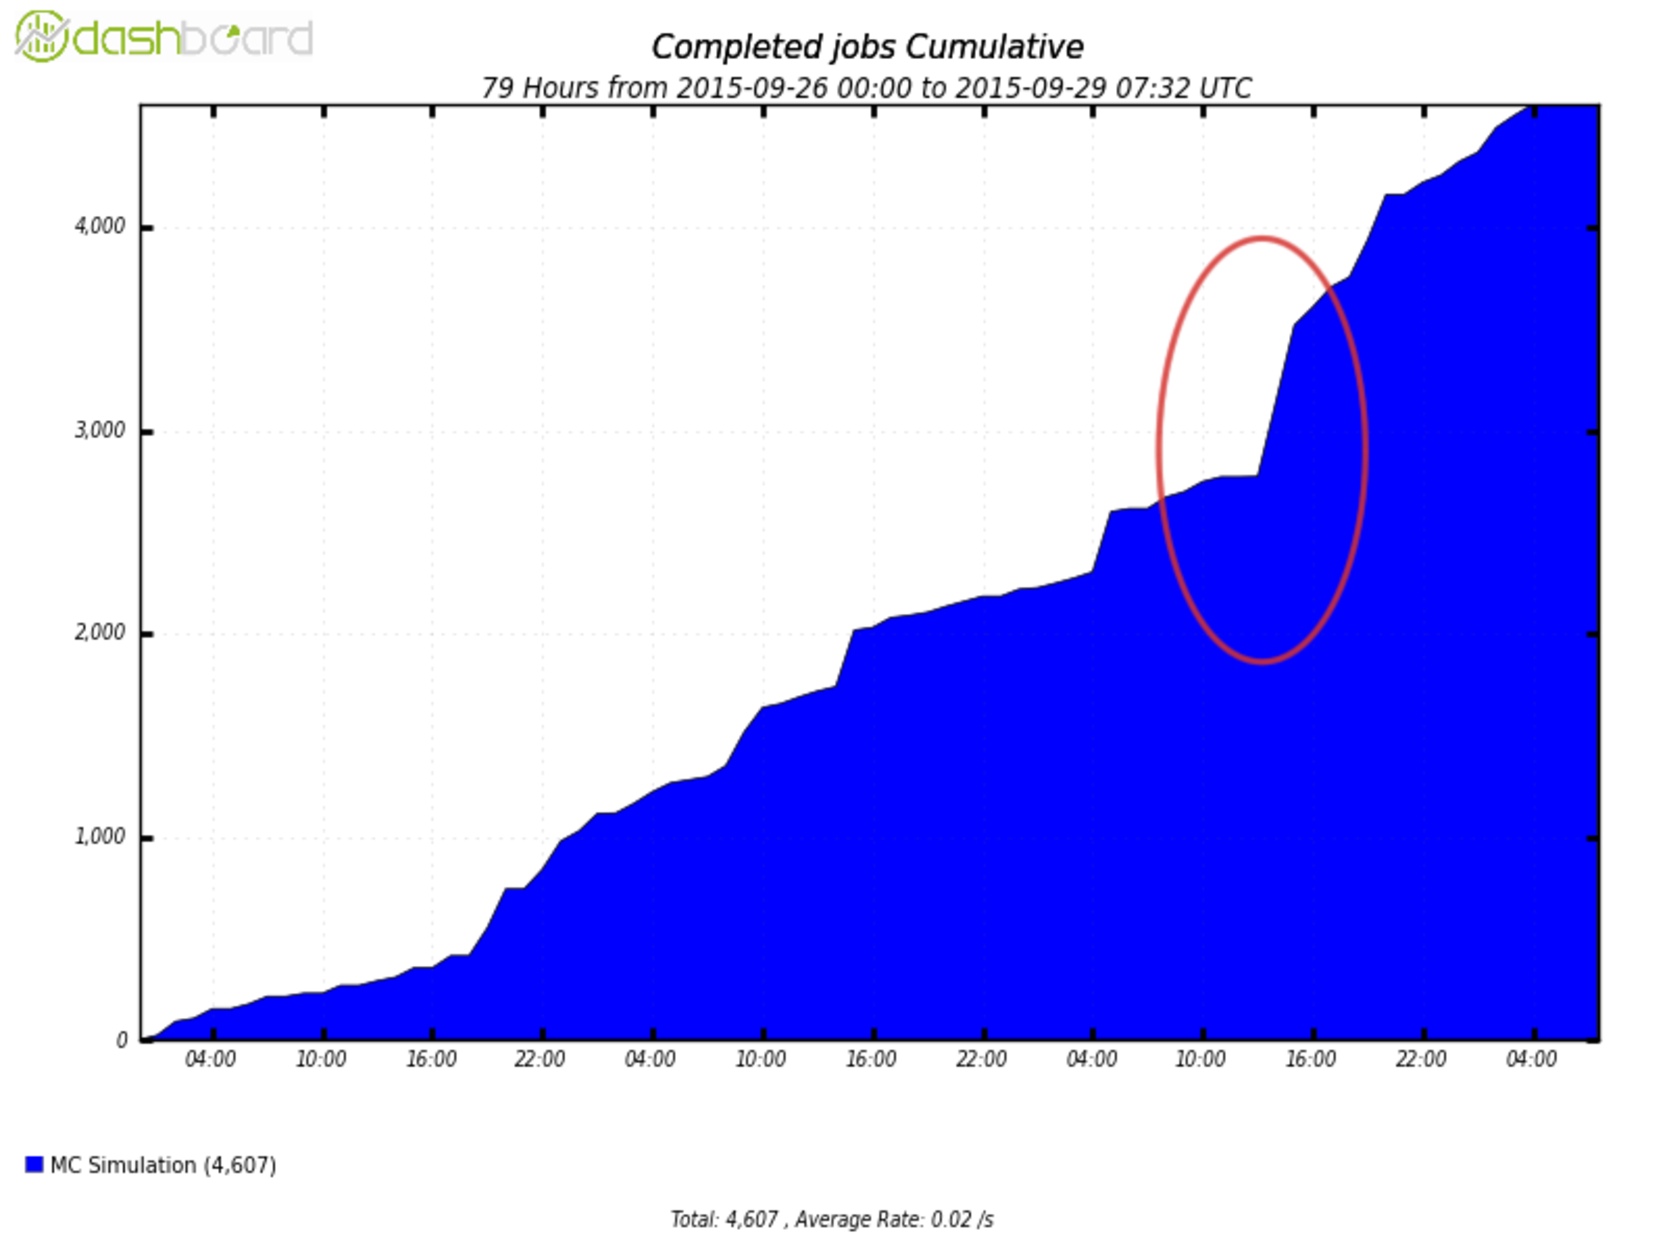
\includegraphics[width=0.48\textwidth]{figures/panda-completed-jobs-sw-move.pdf}}\\
%    \end{tabular}
%    \caption{ATLAS performance improvement on Titan. The circled region shows the switch from Lustre to NFS-exported directory for hosting the ATLAS release.}
%\label{fig:atlas-perf-improvement}
%\end{figure}

Once set up, AthenaMP is used to execute 16 concurrent Geant4 simulators on each
of Titan's worker node. Geant4 requires to read events descriptions from a
filesystem and simulate them as they would happen within the ATLAS detector. We
characterized both the compute performance of the simulation and the impact of
acquiring event descriptions on the filesystem.

The AMD Opteron 6274 CPU used on Titan has 16 cores, divided into 8 compute
units. Each compute units has 1 floating point (FP) scheduler shared between 2
cores. When using 16 cores for FP-intensive calculations, each pair of cores
competes for a single FP scheduler. This creates the overhead shown in
Figure~\ref{fig:comparison-8-16cores}: the mean runtime per event for 8
concurrent simulations computing 50 events is 10.8 minutes, while for 16
simulations is 14.25 minutes (consistent with the measured distribution of the
duration of event simulation). Despite an inefficiency of almost 30\%, Titan's
allocation policy based on number of worker nodes used instead of number of
cores does not justify the use of 1/2 of the cores available.

\begin{figure}[htp]
    \includegraphics[clip,width=\columnwidth]{figures/tx8_tx16_comparison.pdf}
    \caption{Comparison between distributions of the time taken by a Geant4
    detector simulation to simulate one event when placing 2 simulations (h1) or
    1 simulation (h2) per CPU. 2 simulation use 16 cores per node, 1 simulation
    8, 1 per compute unit. 50 Events; 1 Titan worker nodes; 16 work threads per
    node; 100 events per node.}
\label{fig:comparison-8-16cores}
\end{figure}

The performance analysis of Titan's AMD CPUs for detector simulations helps also
to compare Titan and Grid site performances. Usually, Grid sites exposes
resources with heterogeneous CPU architectures and a maximum of 8 (virtual)
cores per worker node, while Titan's offer an homogeneous 16 cores architecture.
We used the rate of events processes per minute as a measure of the efficiency
of executing the same detector simulation on both Titan or Grid sites.
% Figure~\ref{fig:comparison-titan-grid} compares the efficiencies of Titan to
% the BNL and SIGNET Grid sites, normalized for 8 cores. Effective performance
% per-core at Titan is $\approx$0.57 event per minute, roughly 1/2 of BNL and
% 1/3 of SIGNET performances.
Comparisons of the efficiencies of Titan to  the BNL and SIGNET Grid sites,
normalized for 8 cores, show that the effective performance per-core at Titan is
$\approx$0.57 event per minute, roughly 1/2 of BNL and  1/3 of SIGNET
performances.

% \begin{figure}[htp]
%     \includegraphics[clip,width=\columnwidth]{figures/titan_grid_event_rate.pdf}
%     \caption{Comparison of the event rate for finished jobs at Titan (h1), BNL
%     (h2) and GRIDNET (h3). Titan histogram shows 1/2 of the measured values to
%     account for the core difference between Titan (16) and the Grid sites (8).
%     Performance per core: BNL 1.126; SIGNET 0.885; Titan 0.577.\mtnote{TO BE DELETED.}}
% \label{fig:comparison-titan-grid}
% \end{figure}

The differences in performance between Titan and the BNL and SIGNET Grid sites
are due to the FP scheduler competition and the availability of newer
processors. The CPUs at the Grid sites have one FP scheduler per core and are on
average newer than the CPU of Titan. The heterogeneity of the Grid sites' CPUs
explain the higher performance variance compared to the performance consistency
measured on Titan.

% \mtnote{Figure summarizing job performance on Titan analogous to those
% produced with NGE, as discussed in F2F meeting at Rutgers?}
%
% ----------------------------------------------------------------------------
% \subsection{Reliability of PanDA Broker and Detector Simulations on Titan}
% \label{ssec:reliability}
%
% Figure~\ref{fig:failures-titan} shows a breakdown of the type of failures
% recorded by the PanDA Brokers between January 2016 and February 2017. The
% initial preponderance of unknown failures was progressively addressed by a
% more accurate failure model, specifically tailored to the PanDA Broker and
% Titan. Figure~\ref{fig:failures-titan} also shows the progressive improvement
% of the broker's reliability: In Februrary 2017, errors related to input files
% and initialization were almost eliminated and execution errors were comparable
% to those recorded in January 2017 even if almost twice as many simulations
% were performed (Figure~\ref{fig:backfill-utilization}). The increased amount
% of unknown failure in February indicates that furter work is needed to improve
% the PanDA Broker failure model.
%
% \begin{figure}[htp]
%     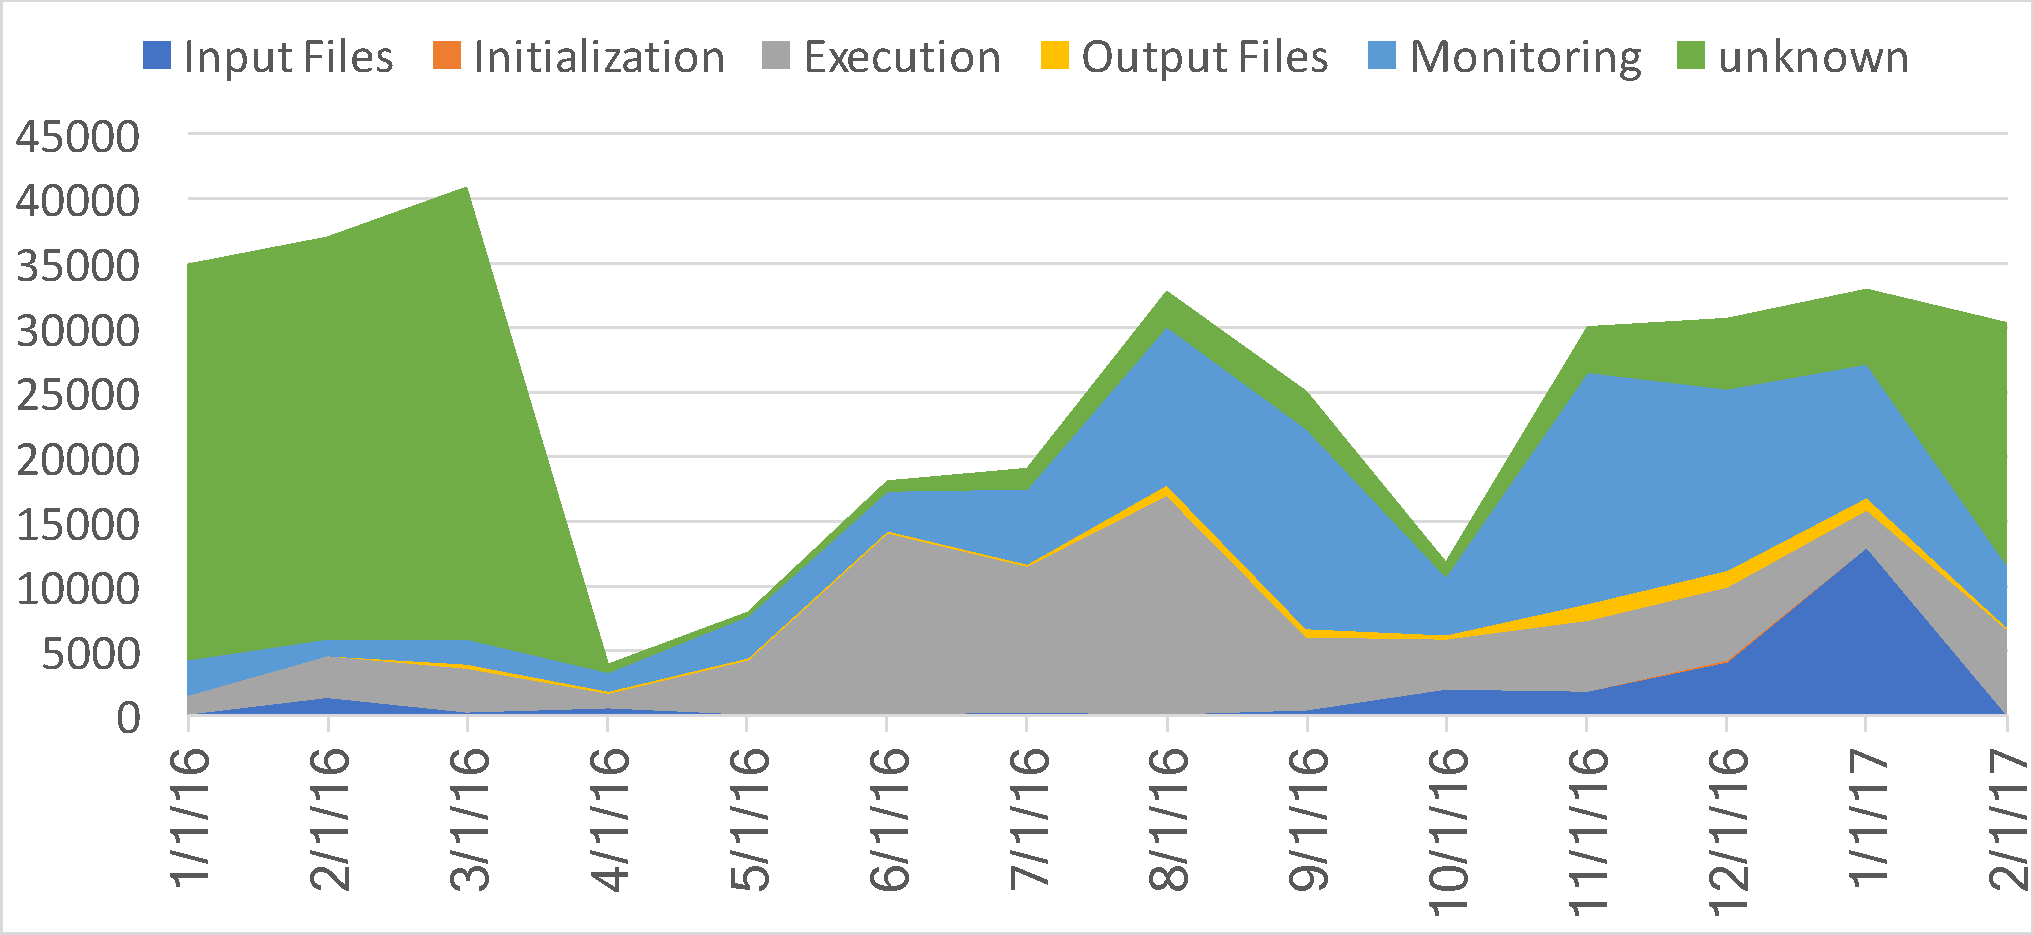
\includegraphics[clip,width=\columnwidth]{figures/failures_titan.pdf}
    % \caption{PanDA Broker failures during the experiment time window. Failures
    % were recorded with 52 exit codes, here aggregated into 6 categories. The
    % number of failures should be compared to the number of simulations
    % executed in each month as plotted in
    % Figure~\ref{fig:backfill-utilization}. Improvements in the failure model
    % of PanDA Broker shows a decrease in unknown failure and a the progressive
    % addressing of other categories of failure.}
% \label{fig:failures-titan}
% \end{figure}
%
% -----------------------------------------------------------------------------
% \subsection{Characterizing PanDA I/O}
%
% To better understand the I/O impact of ATLAS PanDA project on Titan
% supercomputing environment

We studied the impact of acquiring event descriptions on Lustre by analyzing
1,175 jobs ran on the week of 10/25/2016, for a total of 174 hours.
Table~\ref{panda-olcf-stats} shows the overall statistical breakdown of the
observed file I/O.
% Figures~\ref{fig:atlas-titan-io-read} and~\ref{fig:atlas-titan-io-written}
% show the file read and write I/O histograms for these 1,175 jobs,
% respectively. Figures~\ref{fig:atlas-titan-file-open}
% and~\ref{fig:atlas-titan-file-close} show the file $open()$ and $close()$
% metadata load histograms of the same  1,175 ATLAS jobs, respectively.
%
% As can be seen from Table~\ref{panda-olcf-stats},
%
ATLAS used between 1 and 300 worker nodes, and 35 on average. 75\% of the jobs
run by ATLAS consumed less than 25 nodes and 92\% less than 100. During the 174
hours of data collection, 6.75 ATLAS jobs were executed on average per hour,
each job running for an average of 1.74 hours.
% ATLAS jobs issues a large number of file read operations, as can be seen in
% Table~\ref{panda-olcf-stats}.
Every job read less than 250 GB and wrote less than 75 GB of data and, on
average, each job read 20 GB and wrote 6 GB of data.

\begin{table*}[t]
\centering
\begin{tabular}{lllllllll}
 & Num. Nodes & Duration (s) & Read (GB) & Written (GB) & GB Read/nodes & GB Written/nodes & $open()$ & $close()$ \\
Min & 1 & 1,932 & 0.01 & 0.03 & 0.00037 & 0.02485 & 1,368 & 349 \\
Max & 300 & 7,452 & 241.06 & 71.71 & 0.81670 & 0.23903 & 1,260,185 & 294,908 \\
Average & 35.66 & 6,280.82 & 20.36 & 6.87 & 0.38354 & 0.16794 & 146,459.37 & 34,155.74 \\
Std. Dev. & 55.33 & 520.99 & 43.90 & 12.33 & 0.19379 & 0.03376 & 231,346.55 & 53,799.08
\end{tabular}
\caption{The Statistical breakdown of the I/O impact of 1,175 jobs ATLAS executed at OLCF for the week of 10/25/16}
\label{panda-olcf-stats}
\end{table*}

% \begin{figure}[!htb]
%     \centering
%     \begin{tabular}{cc}
%         {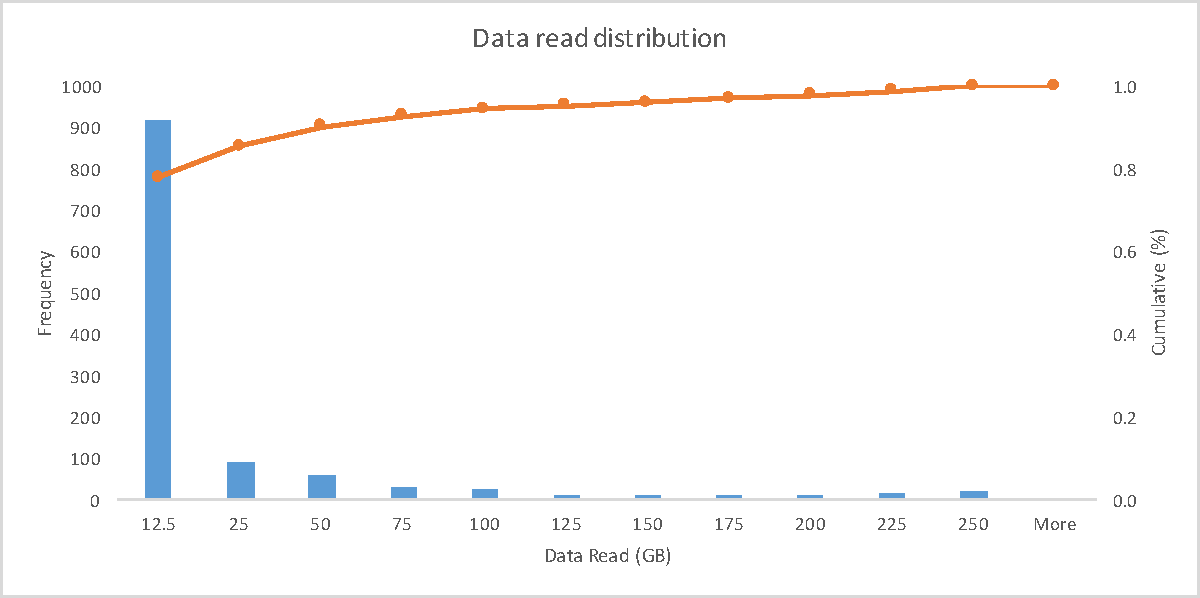
\includegraphics[width=0.48\textwidth]{figures/panda_data_read_finer_hist.pdf}}\\
%     \end{tabular}
%     \caption{ATLAS file read operation histogram on Titan for week of 10/25/16.}
% \label{fig:atlas-titan-io-read}
% \end{figure}
%
% \begin{figure}[!htb]
%     \centering
%     \begin{tabular}{cc}
%         {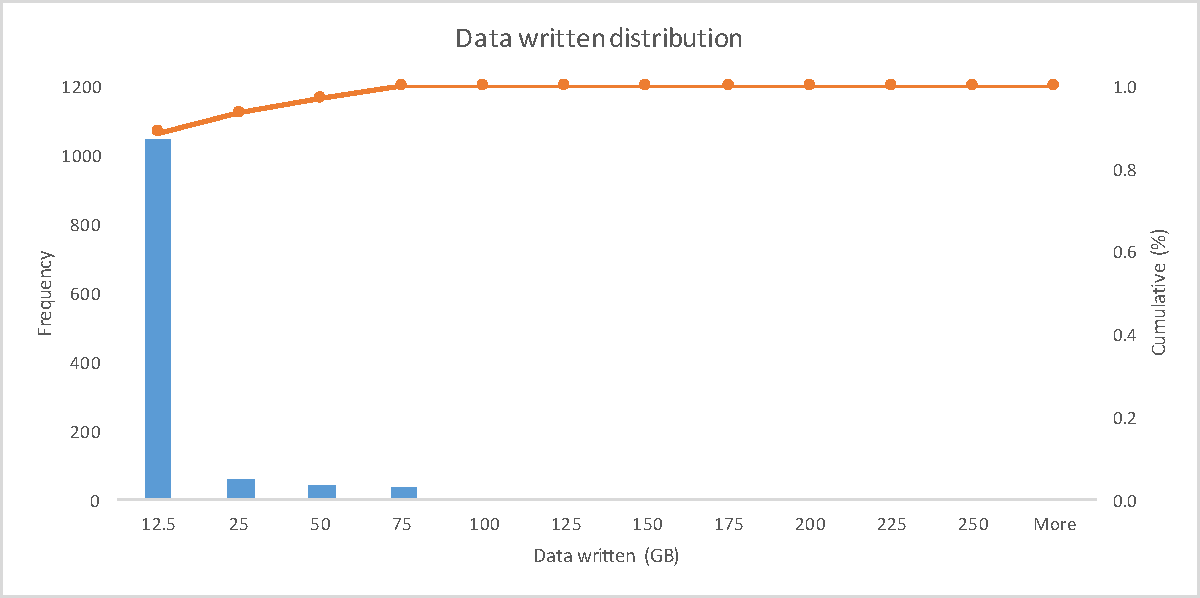
\includegraphics[width=0.48\textwidth]{figures/panda_data_written_finer_hist.pdf}}\\
%     \end{tabular}
%     \caption{ATLAS file write I/O histogram on Titan for week of 10/25/16.}
% \label{fig:atlas-titan-io-written}
% \end{figure}

% The I/O of the ATLAS jobs show an interesting pattern.
% Table~\ref{panda-olcf-stats} indicates that the amount of data read per ATLAS
% worker node is less than 400 MB on average, while the amount of data written
% per node is less than 170 MB on average. This correlates with our finding
% that ATLAS PanDA jobs are read heavy. However,

ATLAS jobs are read heavy: On average, the amount of data read per worker node
is less than 400 MB, while the amount of data written is less than 170 MB.
% as can be seen in Table~\ref{panda-olcf-stats} and figures
% {fig:atlas-titan-io-read} and {fig:atlas-titan-io-written},
Distributions of read and written data are different: The read operation
distribution per job shows a long tail, ranging from 12.5 GB to 250 GB, while
the written amount of data has a very narrow distribution.

% \begin{figure}[!htb]
%     \centering
%     \begin{tabular}{cc}
%         {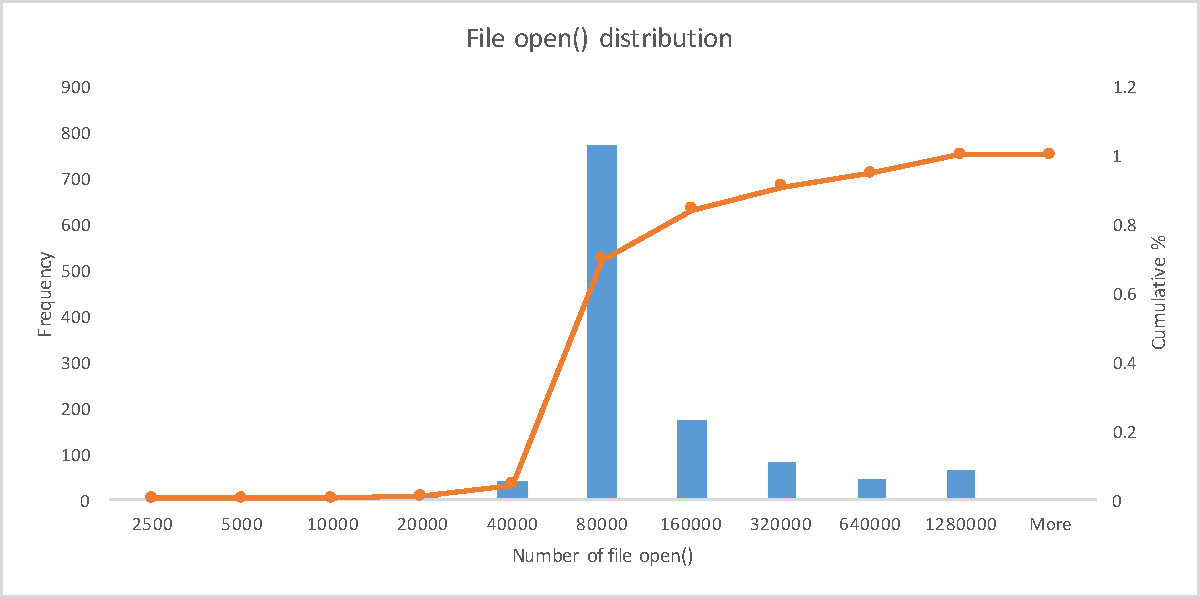
\includegraphics[width=0.48\textwidth]{figures/panda_file_open_hist.pdf}}\\
%     \end{tabular}
%     \caption{ATLAS file $open()$ histogram on Titan for week of 10/25/16.}
% \label{fig:atlas-titan-file-open}
% \end{figure}
%
% \begin{figure}[!htb]
%     \centering
%     \begin{tabular}{cc}
%         {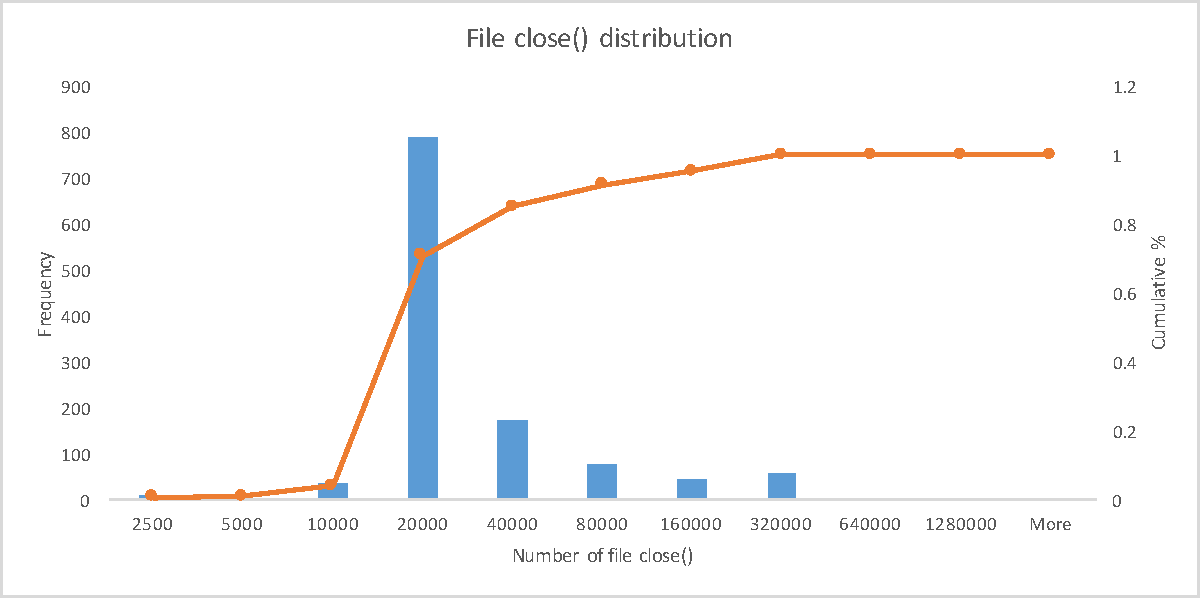
\includegraphics[width=0.48\textwidth]{figures/panda_file_close_hist.pdf}}\\
%     \end{tabular}
%     \caption{ATLAS file $close()$ histogram on Titan for week of 10/25/16.}
% \label{fig:atlas-titan-file-close}
% \end{figure}

The metadata I/O breakdown shows that ATLAS jobs yield 23 file $open()$
operations per second (not including file $stat()$ operations) and 5 file $close()$ operations per second, with similar distributions.
% As can be seen from figures~\ref{fig:atlas-titan-file-open}
% and~\ref{fig:atlas-titan-file-close}, they .
On average, the maximum number of file $open()$ operations per job is
$\approx$170/s and the maximum number of file $close()$ operations is
$\approx$39/s.
% on average per second per job.
For the 1,175 ATLAS jobs observed, the total number of file $open()$ operations
is 172,089,760 and the total number of file $close()$ operations is 40,132,992.
The difference between these two values is still under investigation: One
possible explanation is that ATLAS jobs don't call a file $close()$ operation
per every file $open()$ issued.

% based on our experiments with ATLAS jobs, it can be safely concluded
% that the file and metadata I/O load of ATLAS PanDA project on the OLCF Titan
% supercomputing environment and the Spider 2 file system is not detrimental to
% the center operations. At the current scale of the project, the overall impact
% of ATLAS operations on Titan is minimal.

Overall, the average time taken to read events from input files stored on Lustre is 1,320, comparable to the time taken to read the file required by assembling AthenaMP from NFS. Preliminary investigation shows that this time could be reduced to 40 seconds by loading the event descriptions into the RAM disk available on each worker node. Events descriptions could be transferred from Lustre to the RAM disk while configuring and initializing AthenaMP, almost halving the time currently required by initiating a Genat4 simulation.

The current design and architecture of the PanDA Broker is proving to be as
reliable as PanDA Pilot when used on the WLCG. Between Jan 2016 and Feb 2017,
the overall failure rate of all the ATLAS detector simulation jobs was 14\%,
while the failure rate of jobs submitted to Titan was a comparable 13.6\%. PanDA
Brokers were responsible for around the 19\% of the failures, compared to the
29\% of failures produced by the JobDispatcher module of the PanDA Server, and
the 13\% failures produced by the Geant4 toolkit. The current failure rate of
the PanDA Brokers confirms the benefits of reusing most of the code base of the
PanDA Pilot for implementing the PanDA Broker. It also shows that adopting
third-party libraries like RADICAL-SAGA did not have a measurable adverse effect
on reliability.
